
\section{Generalization} 
\subsection{subsec} % this enables bulletpoints at the top of the slide

\begin{frame}
    \frametitle{Generalization - Idea}
    \begin{itemize}
    	\item State-spaces often large
    	\item Calculate utilities with parameters $\theta$
    	\item Function approximation
    	\item Learn parameters instead of utilities
	\end{itemize}
	
	\begin{tikzpicture}
	\node[draw,text width=10cm] (approximation) at (0,0) {
	\begin{equation*}
		\hat{U}_{\theta}(s) = \theta_{1}f_{1}(s) + \theta_{2}f_{2}(s) + \cdots + \theta_{n}f_{n}(s)
	\end{equation*}
	};
	\end{tikzpicture}
\end{frame}

\begin{frame}
    \frametitle{Generalization - Example}
    \begin{itemize}
    	\item Grid world of size 20x20.
    	\item Goal state +1 in position (10,10)
	\end{itemize}

	\begin{tikzpicture}
	\node[draw,text width=10cm] (example) at (0,0) {
	\begin{equation*}
		\hat{U}_{\theta}(s) = \theta_{1}f_{1}(x,y) = \theta_{1}\sqrt{(x-10)^2 + (y-10)^2}
	\end{equation*}
	};
	\end{tikzpicture}
	
	\begin{center}
		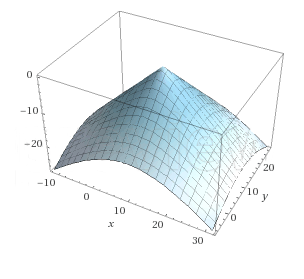
\includegraphics[width=0.4\linewidth]{img-michael/generalization_cone.png}
	\end{center}
\end{frame}

\begin{frame}
    \frametitle{Generalization - Update rule}
    \begin{itemize}
    	\item Widrow-Hoff rule or Delta rule
    	\item Adjust parameters after each trial
    \end{itemize}
    
	\begin{tikzpicture}
	\node[draw,text width=10cm] (update_rule) at (0,0) {
	\begin{equation*}
		\theta_{i} \leftarrow \theta_{i} - \alpha \frac{\partial E_{j}(s)} {\partial\theta_{i}}
	\end{equation*}
	};
	
	\node[draw,text width=10cm] (update_rule_sub) at (0,-2) {
	\begin{equation*}
		E_{j}(s) = \frac{(\hat{U}_{\theta}(s) - u_{j}(s))^2} {2}
	\end{equation*}
	};
	\end{tikzpicture}
	
    \begin{itemize}
    	\item $u_{j}(s)$: observed utility of state s in j-th trial
    	\item $\alpha$: learning factor
    	\item Leads to hill-climbing
    \end{itemize}
\end{frame}

\section{Policy Search} 
\subsection{subsec} % this enables bulletpoints at the top of the slide

\begin{frame}
    \frametitle{Policy Search - Idea}
    \begin{itemize}
    	\item Find a policy $\pi_{\theta}$ for state-space
    	\item Represent policy as parameterized formula
    	\item Like generalization, but parameters for action choice instead of utility calculation
    	\item Obvious policy: choose action which promises biggest reward $\rightarrow$ greedy agent
    \end{itemize}
\end{frame}

\begin{frame}
    \frametitle{Policy Search - Problems}
    \begin{itemize}
    	\item  $\pi_{\theta}$ often discontiuous function
    	\begin{itemize}
    		\item Slightly changed parameters $\rightarrow$ choose another action
    		\item Impossible to take derivative
    	\end{itemize}
    \end{itemize}
    
	\begin{center}
		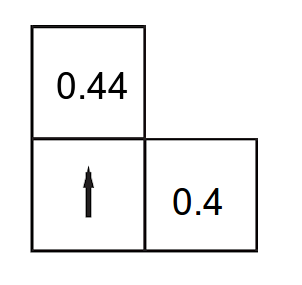
\includegraphics[width=0.3\linewidth]{img-michael/policy_search_first_choice.png}
		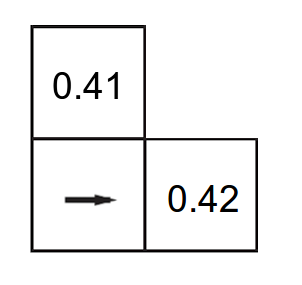
\includegraphics[width=0.3\linewidth]{img-michael/policy_search_second_choice.png}
	\end{center}
	
    \begin{itemize}
    	\item Example: greedy agent
	\end{itemize}
\end{frame}

\begin{frame}
	\frametitle{Policy Search - Problems}
	\begin{itemize}
    	\item Solution: stochastic policy representation
    \end{itemize}
    
    Softmax function:
    
	\begin{tikzpicture}
	\node[draw,text width=10cm] (softmax) at (0,0) {
	\begin{equation*}
		\pi_{\theta}(s,a) = e^{Q_{\theta}(s,a)}/\sum_{a'}e^{Q_{\theta}(s,a')}
	\end{equation*}
	};
	\end{tikzpicture}
	
	\begin{itemize}
    	\item $\pi_{\theta}(s,a)$: probability of taking action a in state s
    	\item $Q_{\theta}(s,a)$: expected utility of taking action a in state s
    \end{itemize}
\end{frame}

\begin{frame}
	\frametitle{Policy Search - Policy Improvement}
	\begin{itemize}
    	\item How to evaluate policy?
    	\item Policy value $\rho(\theta)$
		\begin{itemize}
    		\item Expected reward for executing policy $\pi_{\theta}$
    	\end{itemize}
    	\item Follow policy gradient $\nabla_{\theta}\rho(\theta)$
		\begin{itemize}
    		\item Standard optimization problem
    	\end{itemize}
    \end{itemize}
\end{frame}

\begin{frame}
	\frametitle{Policy Search - Policy Improvement}
	\begin{itemize}
    	\item $\rho(\theta)$ often not differentiable
		\begin{itemize}
    		\item Execute policy $\pi_{\theta}$
    		\item $\rho(\theta) = $ accumulated reward of trial
    		\item Observe change of $\rho(\theta)$ for small changes of $\theta$
    		\item Pick change with biggest improvement of $\rho(\theta)$
    	\end{itemize}
    \end{itemize}
    
	\begin{center}
		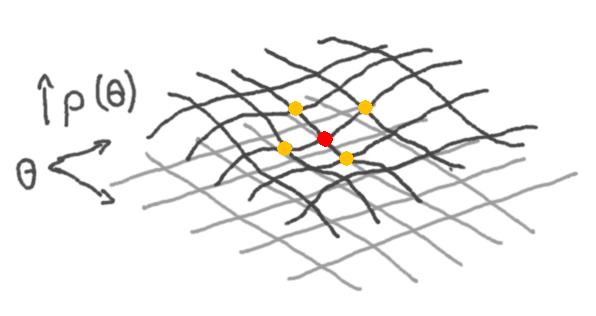
\includegraphics[width=0.6\linewidth]{img-michael/hill_climbing.png}
	\end{center}
\end{frame}

\begin{frame}
	\frametitle{Policy Search - Policy Improvement}
	\begin{itemize}
    	\item Problematic in stochastic environment (same policy, different outcome)
		\begin{itemize}
    		\item Run several trials and take average
    	\end{itemize}
    	\item Trials might be expensive or dangerous
		\begin{itemize}
    		\item Obtain estimate of $\nabla_{\theta}\rho(\theta)$ by looking at $R(a)$
    		\item $R(a)$: sum of subsequent rewards in trials where we chose action a
    	\end{itemize}
    \end{itemize}
	\begin{tabular}{C{5.5cm}  L{4cm}}
		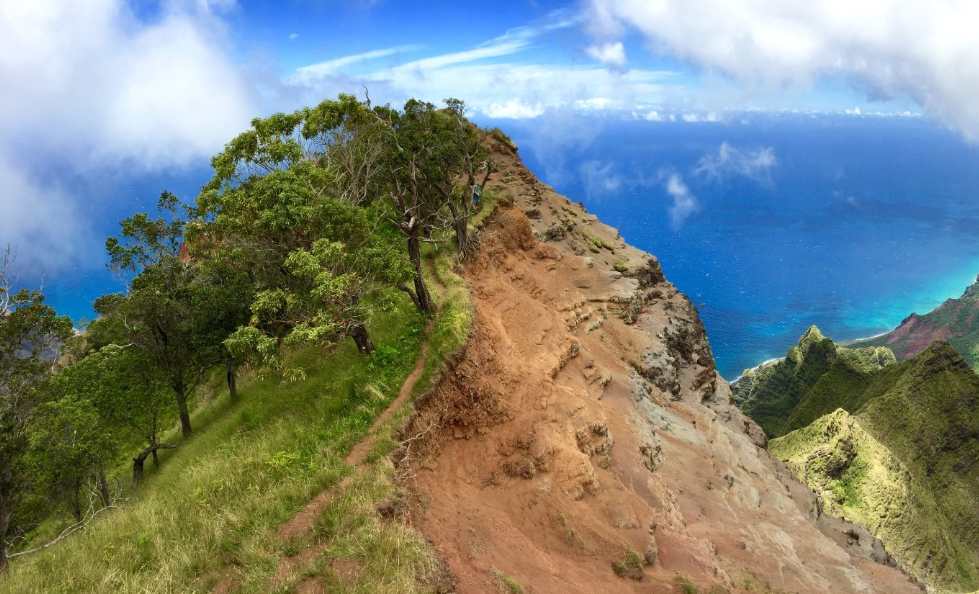
\includegraphics[width=\linewidth]{img-michael/mountain_ridge.png} & It would be dangerous for an agent to go for hundreds of hikes on a ridge of a mountain.\blfootnote{Image source: www.tripadvisor.ch}
	\end{tabular}
\end{frame}

\section{Summary}
\subsection{subsec} % this enables bulletpoints at the top of the slide

\begin{frame}
	\frametitle{Summary}
	\begin{itemize}
		\item Different ways of designing agents:
		\begin{itemize}
			\item Learn passively / actively
			\item Assign utitlies to states or state-action pairs
		\end{itemize}
		\item Many different algorithms for learning
		\begin{itemize}
			\item All converge to Bellmann equation with different speeds
		\end{itemize}
		\item Difficulty of balancing exploration and exploitation
		\item Environments can have huge numbers of states:
		\begin{itemize}
			\item Generalize utility estimation
			\item Generalize policy
			\item Learn parameters instead of directly learning utilites
		\end{itemize}
    \end{itemize}
\end{frame}

\begin{frame}
	\frametitle{Questions}
	Questions?
\end{frame}